Article: Modelling Recurrent Events for Improving Online Change Detection.

\begin{abstract}
The task of online change point detection in sensor data streams is often complicated due to presence of noise that can be mistaken for real changes and therefore affecting performance of change detectors.
Most of the existing change detection methods assume that changes are independent from each other and occur at random in time.
In this paper we study how performance of detectors can be improved in case of recurrent changes.
We analytically demonstrate under which conditions and for how long recurrence information is useful for improving the detection accuracy.
We propose a simple computationally efficient message passing procedure for calculating a predictive probability distribution of change occurrence in the future. We demonstrate two straightforward ways to apply the proposed procedure to existing change detection algorithms.
Our experimental analysis illustrates the effectiveness of these approaches in improving the performance of a baseline online change detector by incorporating recurrence information.
\end{abstract}

\section{Introduction}
Increasing volumes of data are being generated by sensors when monitoring industrial processes, traffic, or infrastructure.
Such streaming data typically needs to be analyzed continuously as it arrives, using only information observed so far.
Predictive models, once learned on historical data, may become obsolete due to changes in physical process generating data, as well as external changes in the environment.
In machine learning and data mining changes in the underlying data distribution over time are referred as concept drift~\cite{Widmer96}.

A popular approach for handling concept drift is to monitor data or model performance for changes and to adapt model using most recent data collected after the last detected change~\cite{GamaACMCS2014}.
Even without automated model adaptation, online change detection is practically relevant in many domains, such as medicine, energy production, industrial processes monitoring~\cite{Nikiforov}, for signalling human experts that something has changed in the process.

Change points are defined as moments in time, when the statistical properties of a data stream change significantly according to predefined criteria.
The process of online change detection is often challenging due to presence of noise that, when operating online, may be mistaken for real changes.
A good change detector is expected to detect changes within an acceptable time lag, and be robust to noise by not raising false alarms.
A balance between these two requirements is determined by the parameter settings for the detector.
Typically, the optimal settings are learned during an offline training phase, and then applied on newly arriving data.
Our idea is to adjust the sensitivity of the detector online during operation, in relation to the current probability of change reoccurrence.

While many change detection methods have been developed~\cite{Nikiforov,Polunchenko2011} for offline and online settings, they typically assume that changes occur at random in time, and are independent from each other.
In practice, however, in many industrial applications changes occur with some regularity (e.g. seasonality).
Our approach is to capture this information from data, and utilize it for improving the accuracy of online change detection.

Consider the following example.
A continuously operating power production plant needs to be regularly refueled.
Change detection software is deployed for detecting refueling events from sensor data, and providing this information to the operation and control system.
If, for instance, historical data suggests that refueling usually happens between 7pm and 10pm every day, this information can be learned from data, and the sensitivity of the detector can be increased within this time range expecting to improve detection speed, and lowered otherwise expecting to reduce the rate of false alarms.

In this study we analyze how and under which conditions the performance of online change detectors can be improved for detecting recurrent changes:
\begin{itemize}	\setlength\itemsep{0pt}
    \item We define a predictive change confidence function (PCCF) for modelling recurrent changes and predicting times of changes in the future. We derive the exact analytical expression for PCCF under Gaussian data distribution.
    \item We demonstrate under which conditions taking into account recurrence information improves detection accuracy by analytically relating PCCF and time passed from the most recent confirmed change.
%Thus, we show that in case of no feedback or long delay in providing feedback on true changes, the information about past changes is hard to make use of even when there is a strong regularity in recurrence of changes.
%We show that is a confirmation that a change point was detected correctly comes with a considerable delay (or does not come at all), the information about past changes is hard to make use of even when there is a strong regularity in recurrence of changes.

    \item We demonstrate how to improve the accuracy of an online change detector of user's choice by utilizing recurrence information with two simple yet generic approaches: (1)~a post-filtering of change detection output can substantially reduce the number of false alarms while preserving the same detection rate; (2)~an adaptation mechanism can be used to adjust the sensitivity of the detector online based on the change recurrence expectations.

    \item Our experimental study provides evidence that it is indeed feasible to improve performance of online change detection by utilizing recurrence information even with such simple approaches.
\end{itemize}

%\emph{Related work.}
%\section{Related work}
Several lines of work relate to our approach via attention to recurrent concept drift~\cite{GamaK11,DBLP:journals/tnn/GomesGSR14,DBLP:journals/ida/GomesSR12}, predictability of concept drift~\cite{Ang2013}, or change detection with delayed labeling~\cite{DBLP:conf/icdm/Zliobaite10}.
These approaches are specific to handling concept drift, while our focus is on generic online change detection and its accuracy.
%The close approach to ours is
In the Bayesian online change detector proposed in~\cite{mackay2007} and extended in~\cite{ Wilson2010a} authors model time intervals between change points (run lengths) using the hazard rate.
This approach allows to take into account recurrence by tuning single parameter, but it does not allow to distinguish outliers from changes which may appear between them.
In~\cite{huang2014detecting} data stream volatility, defined as the rate of detected changes, is used to make detector more reactive.
%, which is aimed at capturing episodic reoccurrences, as opposed to modeling reoccurrences in the long run.
We concentrate on the problem of improving change detection  by predicting time locations of the changes in the future in order to better distinguish outliers from real changes.
To the best of our knowledge this is the first work that explicitly models change recurrence as PCCF and uses it to enhance online change detection performance.

\emph{Outline.} The rest of the paper is organized as follows.
In Section~\ref{sec:chpprocess} we describe an individual change detection procedure and give definitions for recurrent and periodic changes.
In Section~\ref{sec:predictionprocess} we describe our approach for computing PCCF. %online detection of recurrent changes.
In Section~\ref{sec:pccf_integration} we describe integration of PCCF with a base-level change detector.
In Section~\ref{sec:experiments} we summarize the results of our experimental study.
Section~\ref{sec:conclusions} concludes the paper with the summary of the contributions and future work.

%\section{Online change detection process}
\section{Recurrent and periodic changes}
\label{sec:chpprocess}
The purpose of the change detection process is to detect changes in the input data stream of observations $x_t, t \in \T$ to be obtained sequentially at time moments $\T=\Collect{t_1,t_2,\dots,t_T} \equiv \Collect{t_q}_{q=1}^T$ with a constant sampling rate.
Change is identified by the moment of time when it happened.
%Let us denote the sequence of changes to be detected within $\delta$ lapse as $\Collect{c_i }_{i=1}^k \in \T$ and an individual change from this sequence as $c_i$.
Let us denote the sequence of changes to be detected as $\Collect{c_i }_{i=1}^k \in \T$ and an individual change from this sequence as $c_i$.
After a change occurs, we need to collect a new portion of observations during the time $\delta$ to detect the change and to assess a new probability distribution of the data.

Change detector can be considered as a binary classifier whose output for each $x_t$ is the label $\lbl{+}$ if change is alarmed, which we call a change detection event (CDE) and denote it $\Event{t}{+}$, and label $\lbl{-}$ otherwise, which we denote as  $\Event{t}{-}$.

To assess detectors' performance we define True Positive (TP), False Positives (FP), True Negatives (TN) and False Negatives (FN) as follows:
\begin{itemize}[leftmargin=*]\setlength\itemsep{0em}
    \item $\Event{t}{+}$ is TP if $\exists c_i:t-c_i<\delta$, and FP if $\nexists c_i:t-c_i<\delta$
    \item $\Event{t}{-}$ is FN if $\exists c_i:t-c_i <\delta$, and TN if $\nexists c_i:t-c_i<\delta$
\end{itemize}
%\begin{itemize}[leftmargin=*]\setlength\itemsep{0em}
%    \item $\Event{t}{+}$ is TP if $\exists c_i:|c_i-t|<\delta$, and FP if $\nexists c_i:|c_i-t|<\delta$
%    \item $\Event{t}{-}$ is FN if $\exists c_i : |c_i-t| <\delta$, and TN if $\nexists c_i:|c_i-t| < \delta$
%\end{itemize}
%We use modulus because an actual change takes some time and is usually identified by a time moment in the middle of the transition phase with duration $2 \delta$.

Recall the real world example of a power production plant, where the task is to detect changes in the fuel mass flow signal generated by monitoring sensors.
One subtask is to detect online changes in the signal that correspond to the refueling process~\cite{PechenizkiySIGKDDExpl09}.
Consider two scenarios.
Scenario \textbf{A}: historical data indicates that refueling typically happens every day in between 7pm and 10pm (90\% of all the observed cases).
Hence, if a detector alarms a change at 11am we may conclude that most likely it is an outlier and take actions to prevent FP.
Scenario \textbf{B}: we have information that refueling is performed only when the fuel is about to run out, but we have no information that % refueling
it is performed on a daily basis.
We can observe from historical data that the average time between refueling  events is between 32 and 36 hours (90\% of all observed cases).

The two scenarios differ in possibilities to anticipate the next change point.
In scenario \textbf{A} we assume that changes are associated with time moments, which can be learned and thus known in advance (e.g.\ end of the day), while in scenario \textbf{B} we can relate future changes to the recently detected event(s).
Nevertheless, in both cases our intuition is to estimate the average time between changes from historical data, and use this information for determining the time periods where changes are more likely to happen in the future.

Let us denote by $p(c|\theta)$ a probability mass function (Pmf) defined on a discrete set of time moments $\T$ parameterized by vector $\theta$ holding information about expected distance between consecutive changes (e.g.\ the average and standard deviation).
By $p(c_i=t|\theta)$ we denote Pmf for a change $c_i$ to happen at time $t$. Recurrent and periodic changes are defined as follows.
\begin{definition}
\label{def:periodicdefinition}
Changes $\Collect{c_i}_{i=1}^k$ are periodic if
\begin{equation}
p(c_{i+1} = t|\theta) = p(c_1 = t - i w \: | \: \theta), i \in \mathbb{Z},
\label{eq:procwithrefs}
\end{equation}
where $c_1$ is the time of the first change and $w$ is a time range within which we expect the next change.
\end{definition}
Definition~\ref{def:periodicdefinition} corresponds to the case \textbf{A} and states that Pmf of a periodic change $c_{i+1}$ is a Pmf of the change $c_1$ shifted along the time axis by  $i w$.
In the power plant example, refueling happens every day in the evening, i.e.\ $i w$ is the beginning of the $i^{th}$ day and $w = 24$ hours.
%Definition~\ref{def:periodicdefinition} corresponds to the case \textbf{A} and states that Pmf of $(i+1)^{th}$ periodic change is a Pmf of the $1^{st}$ change shifted along the time axis by  $i w$. In the power plant example refueling happens every day in the evening, i.e.\ $i w$ is the beginning of the $i^{th}$ day and $w = 24$ hours.
\begin{definition}
\label{def:recurrentdefinition}
Changes $\Collect{ c_i }_{i=1}^k$ are recurrent if
\begin{equation}
p(c_{i+1} = t \: | \: \theta) = p(c_1 = t - c_{i} \: | \: \theta),
\label{eq:procnorefs}
\end{equation}
where
$c_1$ is the time of the $1^{st}$ change and
$c_i$ is the time of the $i^{th}$ change.
\end{definition}
Definition~\ref{def:recurrentdefinition} corresponds to the case \textbf{B} and states that Pmf of the change $c_{i+1}$ is a Pmf of the change $c_1$ shifted along the time axis by time of the $i^{th}$ change $c_i$.

\section{Online detection of recurrent changes}
\label{sec:predictionprocess}
%We can formally define PCCF as follows.
\begin{definition}
\label{def:confidencefunc}
PCCF is the probability to observe \textit{any} a recurrent change out of sequence of all possible changes $c \in \Collect{ c_i }_{i=1}^k$ at any given time moment $t$:
\begin{equation}
\mathcal{P}(t \: | \: \theta) = \sum_{i=1}^{k} p(c_i = t \: | \: \theta).
\end{equation}
% \mathcal{P}(c = t - t_s | \theta) = \sum_{i=1}^{k} p( c_i = t - t_s | \theta), c_i > t_s
\end{definition}
Next we demonstrate how to compute PCCF for recurrent (Scenario \textbf{B}) and periodic (Scenario \textbf{A}) changes, and update it using time stamps of changes $t_s$ confirmed by an online confirmation mechanism.
% {\color{red} offline?} - why?
% !!! Possible can be deleted/commented:
We show under which conditions recurrence information in a form of the average time between changes and its standard deviation $\theta = (\mu, \sigma)$ is beneficial for improving the detection accuracy.

\subsection{PCCF for periodic changes.}
The number of periodic changes $k$, which have happened until now (time $t$), can be calculated using the integer division operation:
\begin{equation}
k = \mathbf{ div }(t,w).
\end{equation}
Using Definition~\ref{def:periodicdefinition}~and~\ref{def:confidencefunc} and omitting $\theta$ we can write
\begin{equation}
\mathcal{P}(t) = \sum_{j=1}^{k = \mathbf{div}(t,w)} p(c_1 = t - (j-1) w).
\label{eq:pccf_periodic}
\end{equation}
If each $p(c_j)$ is defined only within the time interval $(jw-w, j w]$
% $(j w, (j+1) w)$
% {\color{red} maybe better $(j w, (j+1) w )$, inclusive brackets or not}
(e.g.\ $w$ stands for the duration of the day, and we expect every change in a sequence to happen only within the next day) then PCCF will be given only by the last member of the sum in~\Eq{eq:pccf_periodic}.
An example of such PCCF is illustrated in Figure~\ref{fig:periodicexample}.
% ~Eq.(\ref{eq:pccf_periodic})
\begin{figure}[htb!]
\centering
\includestandalone[width=0.40\textwidth]{articles/pics/sdm_paper/PeriodicalEvents}
\caption{
An example of PCCF function for periodic events with $w=24$h, $i w = (24, 48, 72, \dots)$.}
\label{fig:periodicexample}
\end{figure}

\subsection{PCCF for recurrent changes.}
According to Definition~\ref{def:recurrentdefinition} Pmf of the change $c_{i+1}$ is conditioned on the time of the $i^{th}$ change $c_i$.
Following the sum rule for probability\footnote{$P(x) = \sum_{y} P(x|y) p(y)$} in order to compute Pmf of $c_{i+1}$ we need to consider all possible time locations of $c_i$.
\begin{equation}
p(c_{i+1} = t) = \sum_{\tau = i}^{t-1} p(c_{i+1}=t \: | \: c_i = \tau) p(c_i = \tau).
\label{eq:sum_rule_recurrent}
\end{equation}
PCCF is a sum over the total number of possible changes by the time moment $t$:
\begin{eqnarray}
\notag
\mathcal{P}(t) & = &  \sum_{i=1}^{t} \sum_{\tau = i}^{t-1} p(c_{i+1} = t | c_{i} = \tau)  p(c_{i} = \tau) \\
& = & \sum_{i=1}^{t} \sum_{\tau = i}^{t-1}
p(c_{1} = t - c_{i})  p(c_{i} = \tau).
\label{eq:pccf_recurren_1}
\end{eqnarray}

\subsection{Numerical PCCF computation procedure.}
Figure~\ref{fig:cascades} shows a toy example of PCCF calculation for every moment of the recurrent change detection process of time length $T=5$, i.e. $\T=\Collect{1,2,3,4,5}$.
\begin{figure}[htb!]
\centering
\includestandalone[width=0.40\textwidth]{articles/pics/sdm_paper/Cascades}
\caption{
%Trellis structure~\cite{mackay2007}
Possible times of recurrent changes.
Black dots indicate the times at which the $i^{th}$ change may have appeared with non-zero probability.
}
\label{fig:cascades}
\end{figure}
Pmf for the first change $p(c_1) = [p_1, p_2, p_3, p_4, p_5]$ is depicted by the first column of the nodes which are all black since the first change can occur at any moment $t \in [1,5]$.
According to \Eq{eq:sum_rule_recurrent} Pmf for the second change is
%%Equation~\ref{eq:sum_rule_recurrent}
\begin{eqnarray}
\notag
p(c_2) &  =  &\sum_{\tau = 1}^{4} p(c_2 = t | c_1 = \tau) p(c_1 = \tau)\\
& = & \sum_{\tau = 1}^{4} p(c_1 = t - \tau) p(c_1 = \tau).
\end{eqnarray}
This sum can be equivalently written in a matrix form
\begin{equation}
p(c_2) =
\begin{bmatrix}
 p_1 & 0   &  0   & 0   \\
 p_2 & p_1 &  0   & 0   \\
 p_3 & p_2 &  p_1 & 0   \\
 p_4 & p_3 &  p_2 & p_1
\end{bmatrix}
\begin{bmatrix}
p_1\\
p_2\\
p_3\\
p_4
\end{bmatrix}.
\label{eq:second_pccf_matrix}
\end{equation}
Thus, \Eq{eq:second_pccf_matrix} gives Pmf for $c_2$ (second column in Figure~\ref{fig:cascades}).
% % equation~\ref{eq:second_pccf_matrix}
Pmf for $c_3,c_4,c_5$ is calculated using the same procedure.
Finally $\mathcal{P}=p(c_1)+p(c_2)+p(c_3)+p(c_4)+p(c_5)$.
%, PCCF equals to the sum of vectors
The online computation procedure for an arbitrary initial Pmf $p(c_1)$
is described in Algorithm~1. %~\ref{alg:pccfalg}.
%Algorithm~\ref{alg:pccfalg}.

\subsection{The exact PCCF for Gaussian distribution.}
Consider Gaussain distribution for the settings when  $p(x|\theta=(\mu,\sigma)) \sim 0$ for all $x \leq 0$.
%In this section we consider \Ed{the case of} Gaussain distribution for the situations when the condition $p(x|\theta=(\mu,\sigma)) \sim 0$ is satisfied for all $x \leq 0$.

\Eq{eq:sum_rule_recurrent} is a convolution of the Pmf $p(c_1)$ of the $1^{st}$ recurrent change, which is given as a boundary condition, and of the Pmf of the change $c_i$ calculated in the previous step:
\begin{eqnarray} \notag
p(c_{i+1}) & = & (p(c_1) \ast p(c_i)) [\tau] \\
& = & \sum_{\tau = 1}^{t-1} p(c_1 = t - \tau) p(c_i = \tau).
\label{eq:sum_rule_convolution}
\end{eqnarray}
The convolution of two Gaussian distributions (please see the proof in~\cite{bromiley2003products}) is
\begin{equation}
(p(x|\mu_1, \sigma_1) \ast p(x|\mu_2, \sigma_2)) = p(x| \mu_1 + \mu_2, \sqrt{\sigma_1^2 + \sigma_2^2}).
\end{equation}
PCCF for recurrent changes can be written as a t-fold convolution and computed analytically
\begin{equation}
\mathcal{P}(t) =
(
\underbrace{
p(c_1) \ast p(c_1) \ast \dots  \ast p(c_1)
}_\text{t}
)
= p(c_1)^{\ast t}.
\end{equation}
%PCCF for the process of length $T$ is a sum
PCCF for the moment $t$ is a sum
\begin{equation}
    \mathcal{P}(t) = \sum_{l=1}^{t} \frac{1}{\sigma \sqrt{2 \pi l}} \exp \left(\frac{-(t - l \mu)^2}{2 l \sigma^2} \right)
%\mathcal{P}(t) = \sum_{l=1}^{T} \frac{1}{\sigma \sqrt{2 \pi l}} \exp \left(\frac{-(t - l \mu)^2}{2 l \sigma^2} \right)
\label{eq:gaussian_pccf}.
\end{equation}
We can calculate the limit $L$ of $\mathcal{P}(t)$ when $t \to \infty$
\begin{equation}
L = \lim_{t \to \infty} \sum_{l=1}^{\infty} \frac{1}{\sigma \sqrt{2 \pi l}} \exp\left(-\frac{(t- \mu l)^2}{2 l \sigma^2} \right).
%L = \lim_{T \to \infty} \sum_{l=1}^{T} \frac{1}{\sigma \sqrt{2 \pi l}} \exp \left(- \frac{(T  - l \mu)^2}{2 l \sigma^2} \right).
\label{eq:gaussian_pccf_limit}
\end{equation}
We can replace $l$ by $t/\mu$ in the denominators since we are interested in the terms for which $l \sim t / \mu$ and when $t \to \infty$, $\lim_{t \to \infty}\left( \frac{1}{t} - \frac{1}{t/\mu} \right)=0$, we are making approximation error of order $(1 + o(1))$,
%We can replace $l$ by $T/\mu$ in the denominators since we are interested in the terms for which $l \sim T / \mu$ and when $T \to \infty$, $\lim_{T \to \infty}\left( \frac{1}{T} - \frac{1}{T/\mu} \right)=0$, we are making approximation error of order $(1 + o(1))$,
\begin{equation}
L = \lim_{t\to\infty} \sum_{l=1}^{\infty} \frac{\sqrt{\mu}}{\sigma\sqrt{2\pi t}} \exp\left(-\frac{\mu^3 (t/\mu- l)^2}{2t\sigma^2}\right).
% L \approx \frac{1}{\sigma \sqrt{2 \pi T}} \sum_{l=1}^{T} \exp \left(- \frac{\mu^2 (T/\mu  - l)^2}{2 T \sigma^2} \right).
\label{eq:pccf_sum_decomposed}
\end{equation}
Exponential terms corresponding to $l$, for which $|t/\mu - l| \gg \sqrt{t}$, will have small values which we can ignored.
Therefore, we need to estimate the sum consisting of the terms for $l \in [t/\mu \pm \sqrt{t}]$.
It is convenient to consider a wider interval of width $t^{3/5} > \sqrt{t}$.
Let us consider three intervals for $l$
(1) $[0, t/ \mu - t^{3/5})$,
(2) $[t/ \mu - t^{3/5}, t/ \mu + t^{3/5}]$,
(3) $(t/ \mu + t^{3/5}, \infty)$.
The components in the sum in Eq.~\ref{eq:pccf_sum_decomposed} are very small within the intervals (1) and (3) since both are bounded by $\exp(-\frac{\mu^2}{2 \sigma^2} N^{1/5})$.
Therefore, we can find the limit by estimating the sum only within the interval (2):
\begin{equation}
L = \lim_{t\to\infty} \frac{\sqrt{\mu}}{\sigma \sqrt{2\pi t}} \sum_{l=-t^{3/5}}^{t^{3/5}} \exp\left(-\frac{\mu^3 (t/\mu - l)^2}{2t\sigma^2}\right).
%L = \frac{1}{\sigma \sqrt{2 \pi T}} \sum_{i = - T^{3/5}} ^{T^{3/5}} \exp \left(-\frac{\mu^2}{2 \sigma^2} \frac{i^2}{T} \right).
\label{eq:sum_before_integral}
\end{equation}
\Eq{eq:sum_before_integral} is the Riemann sum for the Gaussian integral $\int_{-\infty}^{\infty} e^{-a x^2} dx = \sqrt{\frac{\pi}{a}} $, thus
\begin{equation}
L = \frac{\sqrt{\mu}}{\sigma \sqrt{2\pi}} \int_{-\infty}^{\infty} e^{-\frac{\mu^3 x^2}{2\sigma^2}} dx = \frac{1}{\mu}.
%L = \int_{-\infty}^{\infty} \frac{1}{\sigma \sqrt{2 \pi}} \exp \left(-\frac{x^2 \mu^2}{2 \sigma^2} \right)  = \frac{1}{\mu}.
\label{eq:pccf_limit_proof}
\end{equation}
Figure~\ref{fig:pccf_example} illustrates two Gaussian PCCF functions (Eq.~\ref{eq:gaussian_pccf}) for two cases $(\mu=10, \sigma=2)$ and $(\mu=15, \sigma=3)$.
\begin{figure}[htb!]
\centering
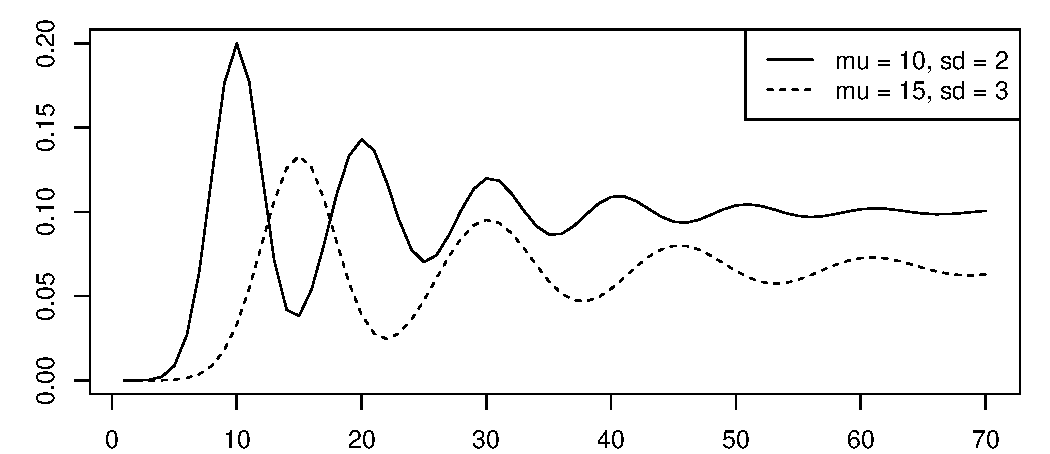
\includegraphics[width=0.40\textwidth]{articles/pics/sdm_paper/pccfExamples.pdf}
\caption{An example of two Gaussian PCCF functions.
}
\label{fig:pccf_example}
\end{figure}
Local extrema of the PCCF function correspond to the time moments $l \mu, l \in \mathbb{Z}$. % where $l$ is a set of positive integers.
PCCF values converge to limits as defined in \Eq{eq:pccf_limit_proof} $L=1/10$ and $L=1/15$.

\subsection{PCCF update after a confirmed change.}
%We consider that the time stamp of the first change is known and initially PCCF is calculated from it.
%After each alarm $\Event{t}{+}$ we need a procedure to reset the detector for next detections.
Typically, a detector would have no internal means to know for sure whether $\Event{t}{+}$ is TP or FP.
If we have a feedback mechanism indicating with some time delay $D$ when a change $c_i$ did happen,
%~\footnote{Please note that this is a delay of confirmation, not  maximum allowed delay of the detection $\delta$.}
we can update PCCF to make our detector more confident about the future change points.
Given a known $c_i$, we recompute PCCF starting from that point.
An updated PCCF is depicted by the dotted line in Figure~\ref{fig:conffunction}.
In Figure~\ref{fig:conffunction} we can see an example of how PCCF oscillates having local maximums at moments $t = k \mu$ until converging to the limit $L=0.1$.
An event at the moment $t=200$ was confirmed as a change and new PCCF is calculated (dashed line).

If we do not reestimate $\theta$ then update procedure is very fast as we simply shift already computed PCCF along the time axis.
% {\color{red} One sentence, what do we conclude?}
\begin{figure}[htb!]
\centering
%\includegraphics[width=0.5\textwidth]{./images/conff3.pdf} \\
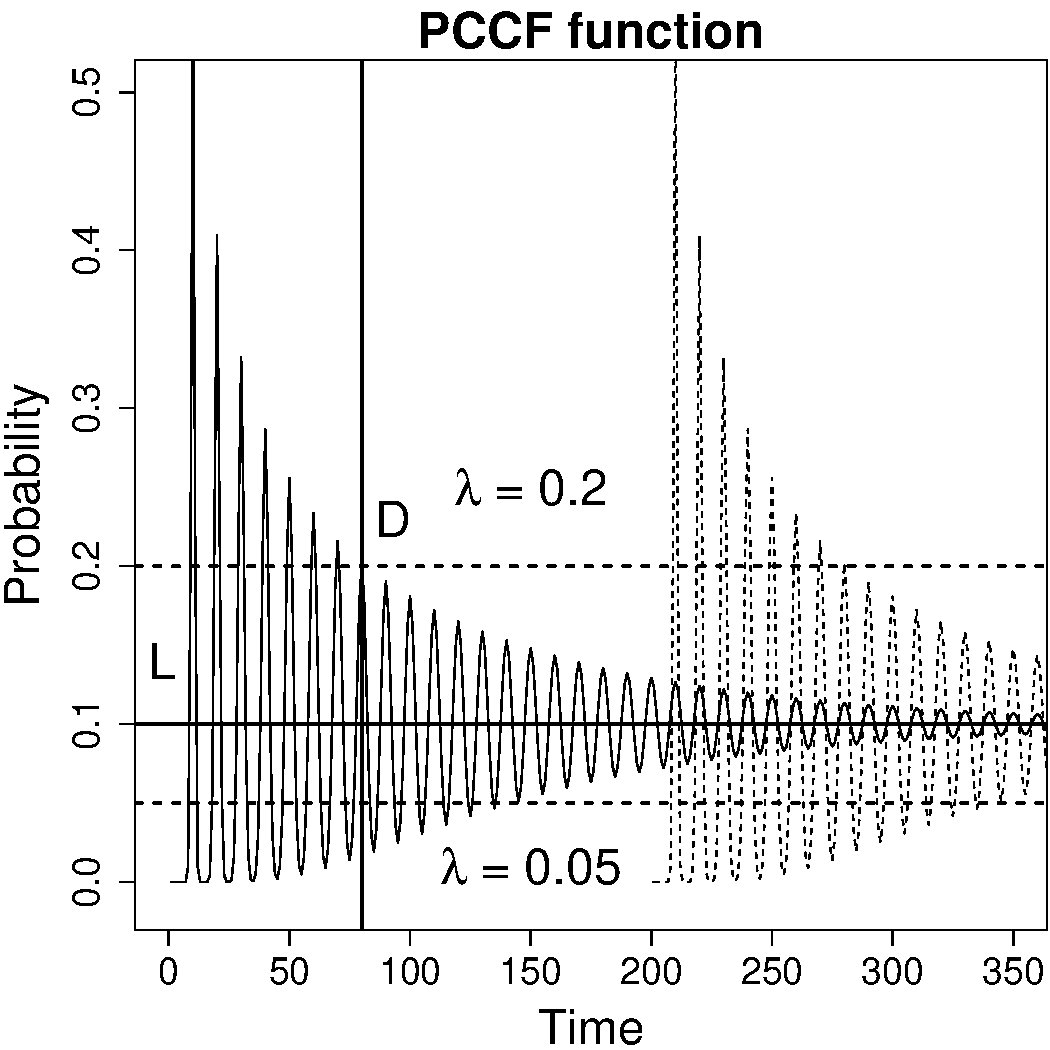
\includegraphics[width=0.35\textwidth]{articles/pics/sdm_paper/PCCF.pdf}
\caption{PCCF converges to the limit $L = 0.1$ depicted by the horizontal bold line.
Two horizontal lines $\lambda$ illustrate possible thresholds above and below the limit.
Vertical line $D$ depicts delay of change confirmation.
%$\lambda$ values illustrate possible threshold values for PCCF.
%$D$ is a maximum allowed delay.
}
\label{fig:conffunction}
\end{figure}

\section{Integration of PCCF into a change detector}
\label{sec:pccf_integration}
%\subsection{Integration of an individual change detector with PCCF}
There are two straightforward approaches for using PCCF can be used to potentially improve the accuracy of existing change detectors:
(1)~post-processing -- a detector with fixed settings is used; its output (CDEs) are adjusted based on PCCFs values,
and (2)~pre-processing -- the sensitivity of the detector is dynamically adjusted according to the current PCCFs values.

At the beginning of the change detection process initial probabilities of changes in the foreseeable future are computed using PCCF.
After that PCCF is recalculated every time the last confirmed $c_i$ is known.

In case of post-processing, a change detector with fixed settings, learned offline, is applied.
When the detector alarms a change at time $t$, we check whether the probability of change given by PCCF is greater than a user defined threshold $\mathcal{P}(t) > p_h$.
If it is, we count CDE as a change and output $\Event{t}{+}$, otherwise we output $\Event{t}{-}$.

In case of pre-processing, detector's settings are adjusted dynamically according to PCCF. The detector is made more sensitive when a change is expected with a higher probability $\mathcal{P}(t) > p_h$, and less sensitive when the change is expected with a lower probability.
This strategy should be applied with caution in order not to make the detector too sensitive, which would result in an increase the FP rate.
In this study we consider only scenario when the highest value of the dynamically adjusted sensitivity of the detector is equal to the optimal threshold value learned during the training phase.
When the estimated probability of the change given by PCCF is low, the sensitivity threshold is lowered.
This scenario is illustrated in Figure~\ref{fig:naivedetector} where detector's sensitivity is a function of PCCF.

\section{Experiments}
\label{sec:experiments}
To illustrate the utility of the PCCF we performed three experiments using artificially generated data and two experiments with real data.
\footnote{We have made the code for computing PCCF and running simulations and experiments publicly available at \url{https://github.com/av-maslov/Pccf}.}.
Our goal is to improve the accuracy of online change detection when recurrent changes are expected.
The required information about recurrence is the time intervals between consecutive changes, given as the parameters of the normal distribution $N(\theta = \mu, \sigma)$.
%After the simulation results, we present the fourth part of the experimental study, in which we demonstrate utility of PCCF on two real data sets.

\subsection{PCCF simulation.}
In order to confirm the correctness of the PCCF Eq.~(\ref{eq:pccf_recurren_1}),~(\ref{eq:gaussian_pccf}) expressing the probability to observe a recurrent change at every moment $t$, we performed a simulation by generating sequences of the recurrent changes multiple times and calculating frequencies of occurrence of generated time locations of the changes at each moment of time.
% (see Algorithm~\ref{alg:pccf_sim} in the appendix).
The shape of the obtained curve of frequencies perfectly fits analytically computed PCCF function.

\subsection{Delay of change confirmation.}
In this simulation we illustrate a procedure to estimate maximum delay of change confirmation $D$ during which the recurrence information in a form of parameters $\theta = (\mu, \sigma)$ is still useful and demonstrate the use of PCCF in post-processing settings.

From Figures~\ref{fig:pccf_example} and~\ref{fig:conffunction} depicting behavior of the PCCF it can be seen that the probability of a change oscillates with decreasing amplitude and converges to the limit $L$.
Assuming the probability of making a FP at any moment is constant and is equal to $\lambda$, there are three scenarios to consider:
\begin{enumerate}
\setlength\itemsep{0pt}
\item The error rate $\lambda$ is higher than $\mathcal{P}(t)$ for all $t$.
In this case the detection accuracy cannot be improved with recurrence information $\theta$;
\item $\lambda$ is higher than the limit $L$ but it is lower than the local maximums of the PCCF $\mathcal{P}(t)$. This case is depicted in Figure~\ref{fig:conffunction} by the horizontal dashed line with value $0.2$.
\item $\lambda$ is lower than the limit $L$; this case is depicted with the horizontal dashed line with value $0.05$.
\end{enumerate}
We are not interested in the first case because the probability of making errors is so high that the baseline change detector should be optimized better first.
In the second case peaks of $\mathcal{P}(t)$ at moments $t = i \mu$ are higher than $\lambda$ until some moment $D$ (vertical line), after which the probability of the error is always higher than the probability of change.
The third case is equivalent to the first case till the moment when local minimums of $\mathcal{P}(t)$ become always larger than $\lambda$.
These observations suggest that we can determine the maximum tolerable confirmation delay $D$ (Figure~\ref{fig:conffunction}) by computing the PCCF function, estimating the error rate of detector, and finding the last peak of $\mathcal{P}(t)$ which is higher than $\lambda$.
To confirm our hypothesis we run the following experiment.

\emph{Input data description}.
For each delay $D$ in the range from 5 to 300 we generate input signal $500$ times with $50$ recurrent change points with $\mu = 10$ and $\sigma = 0.7$.
%The average distance  between changes and its standard deviation are set to $(\mu = 10, \sigma = 0.7)$.
PCCF $\mathcal{P}(t | \mu, \sigma)$ is calculated and updated after the location of the last change is output with the current delay value $D$.
Change point locations are generated according to Definition~\ref{def:recurrentdefinition}, i.e.\ given  $c_1$, the second change is $c_2 = c_1 + \epsilon_1$, $c_3 = c_2 + \epsilon_3$ and so on,  where $\epsilon_i$ is a sample from the Gaussian distribution. %of the first change $p(c_1|\theta = \mu, \sigma)$.
The error rate defining the expected number of FPs per $\mu$ is set to $\lambda = (0.05, 0.2)$.
Time locations of outliers are sampled from the uniform distribution so that there are $1/\lambda$ outliers per time interval of width $\mu$ where $\lambda$ is the FP rate of the detector.

\emph{Change detector.}
In this and the next simulation for PCCF pre-processing we used artificially generated data streams, in which changes are abrupt step changes in the value of the signal.
We use a simple base-level change detector, the output statistic for which is the first order difference of the signal $(x_2  - x_1, \dots, x_n - x_{n-1})$. Its behaviour is illustrated in Figure~\ref{fig:naivedetector}.
A CDE $\Event{t}{+}$ is alarmed when
\begin{equation}
x_i - x_{i-1} > h
\label{eq:naive_detector}
\end{equation}
%
\emph{Experimental results.}
We measure the accuracy of the detector integrated with PCCF for post-processing settings by calculating its TP and FP rates (not the detector it is used to enhance).
The TP rate is a fraction of changes in the input signal that are identified correctly. The FP rate is a fraction of CDEs that would be FPs if the base-level change detector alone was used without PCCF post-processing.
The results are illustrated in Figure~\ref{fig:combined}.
(The corresponding PCCF can be seen in Figure~\ref{fig:conffunction}.)
%The solid black lines in both subfigures depict sensitivity and the dashed line shows specificity of PCCF.

The left plot in Figure~\ref{fig:combined} illustrates the case when periodicity is beneficial for any delay, since the error rate $\lambda=0.05$ is low and $L>\lambda$ almost all the time.
By the time when PCCF converges to its limit
% and the threshold value is below it
all CDEs are considered as changes.
That is why the fraction of correctly predicted changes (bold line) tends to $1$ while the fraction of identified errors tends to $0$ (dotted line).

The right plot illustrates the situation, when recurrence information is beneficial only in some cases, that is when the error rate is lower than the values of PCCF.
The maximum tolerable delay $D$ is illustrated by the vertical line. Please observe that this line is located close to the moments when TP rate goes down \emph{and} FP rate goes up meaning that improvement of the base detector is not possible any more. This confirms our hypothesis that the maximum change confirmation delay $D$ can be estimated by finding the closest local maximum of the PCCF which is higher than $\lambda$.
\begin{figure}[htb!]
\centering
\includestandalone[width=0.45\textwidth]{articles/pics/sdm_paper/artificialsig}
\caption{
	%Output statistic of the naive detector is the first order difference of the signal.
	The base-level detector.
The lower is the threshold the higher is the probability of error.
Outliers between changes $c_1$, $c_2$ and $c_3$ are detected as changes when using constant value threshold $h_1$.
The optimal dynamic threshold is depicted by the dashed line. }
\label{fig:naivedetector}
\end{figure}
%
\begin{figure}[htb!]
\centering
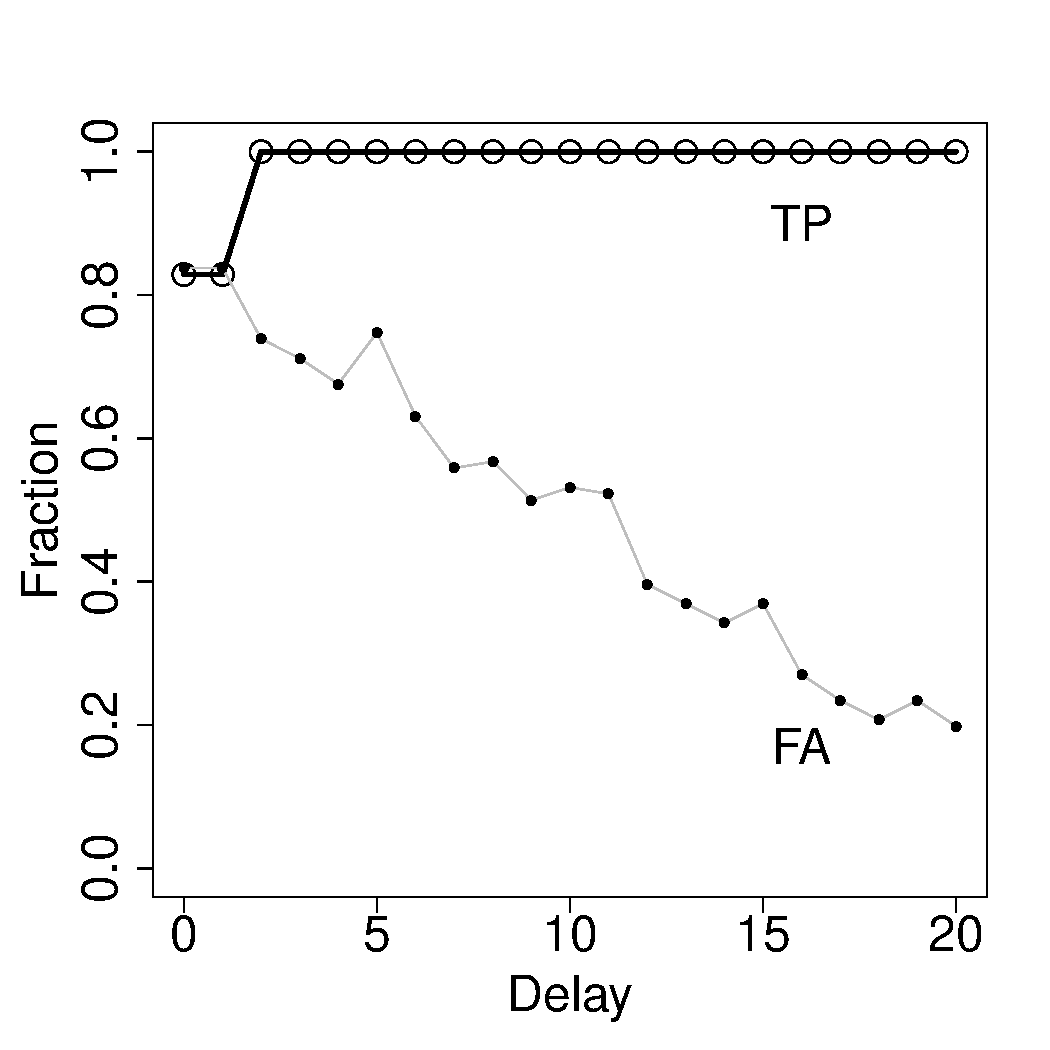
\includegraphics[ width=0.24\textwidth]{articles/pics/sdm_paper/performance2sdm.pdf}
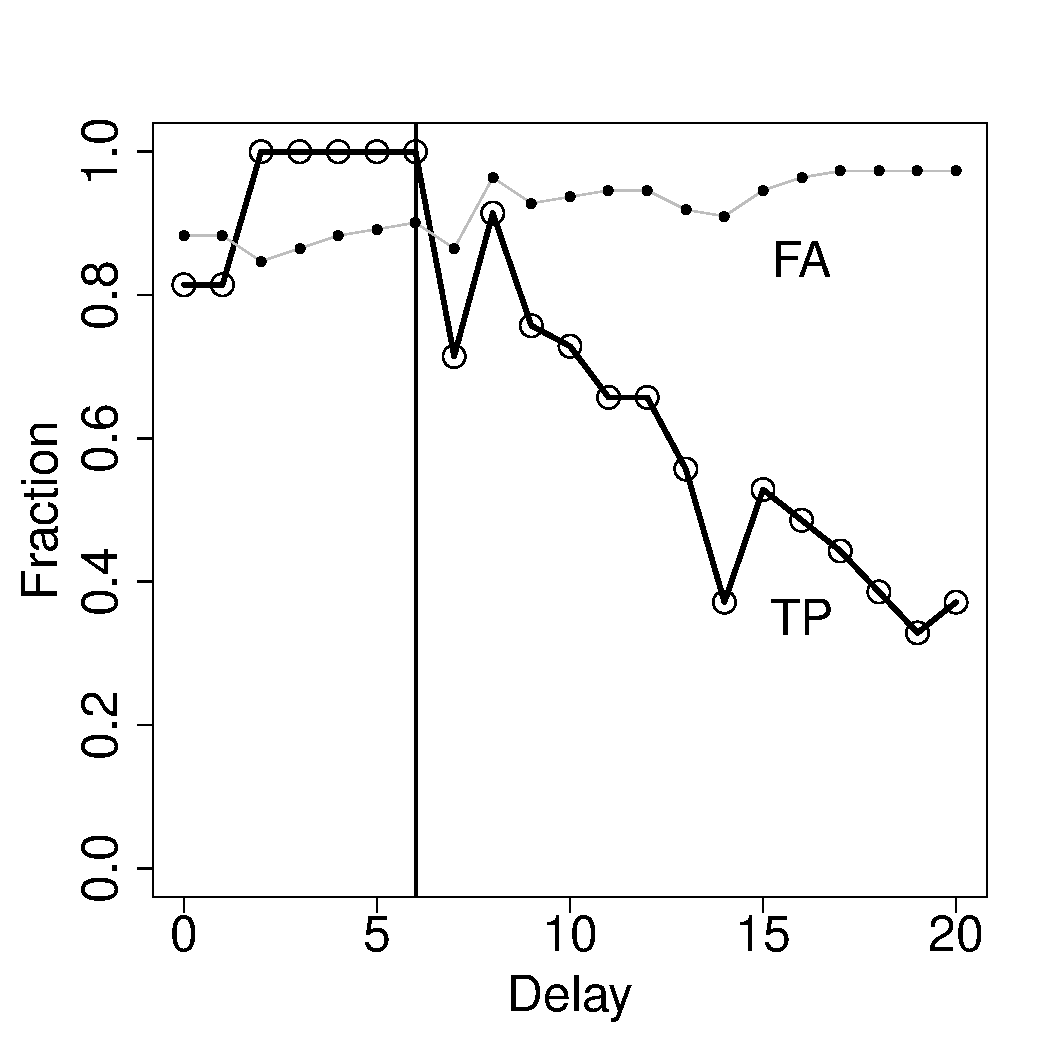
\includegraphics[ width=0.24\textwidth]{articles/pics/sdm_paper/performance1sdm.pdf}
\caption{
% Fractions of CDEs correctly predicted by PCCF as changes (TPs) and error changes (FPs) .
TP and FP rates of PCCF (not the base- or PCCF-enhanced detector) vs. the delay $D$ of change point confirmation.
%in post-processing settings
%by PCCF.
%The sum of TP and FP rates of the base detector would correspond to 1.0.
% {\color{red} Concluding sentence?} - In the text
%Left figure:
%Figure on the top:
%Left figure illustrates the case of the short-term potential usefulness.
%: the error rate $\lambda$ is lower than $\mathcal{P}(t)$ until the vertical line (max delay $D$);
%after that the probability of error is higher.
%This case illustrates the short-term potential usefulness.
%Right figure:
%Figure at the bottom:
% Right figure: the error rate is very low, i.e.\ $L > \lambda$ . %and we detect changes correctly.
}
\label{fig:combined}
\end{figure}

\subsection{Dynamic adjustment of sensitivity.}
This experiment demonstrates the pre-processing approach for integration of PCCF with a change detector, where detection sensitivity is adjusted online.
We first pre-calculate PCCF with parameters $\mu$ and $\sigma$, and then dynamically change the parameters according to the most recent probability of recurrent change.
Recall Figure~\ref{fig:naivedetector} depicting a toy example of dynamically changing threshold $h$ (dashed line).
When PCCF value is low, $h$ is set to a higher value $h_2$, when PCCF value is high, the detector threshold is set to $h_1$.

For this simulation we generate $200$ times input signal with $15$ recurrent changes and $15$ uniformly distributed outliers.
%Locations of the changes and outliers in the signal were generated using the same steps as in the previous simulation,\i.e. recurrent change locations are defined by~\ref{def:recurrentdefinition}, outliers are drawn from uniform distribution with the rate $\lambda$.
The average time interval between changes is $\mu = 10$ with the $\sigma = 0.5$.
The error rate is set to $\lambda = 1$, i.e.\ 1 outlier per time interval of width $\mu$.
% When the error rate is so high, the recurrence information is beneficial, given that the standard deviation is low.
To detect changes we used the same base-level detector as in the previous experiment.

The results are depicted in Figure~\ref{fig:rocdynamic}, showing TP and FP rates.
The performance of the detector without PCCF is depicted by the line with circles, obtained by varying the sensitivity threshold of the detector.
% {\color {red} What do we see?} - we see that (below): We can see that in this case performance of the detector can be improved using PCCF
The performance of the detector with PCCF is depicted by the line with red squares, obtained by changing delay of the $c_i$ confirmation $D$ for a fixed threshold of the base detector.
%Sensitivity of the PCCF based detector was set to the when
We can see that performance of the detector can be improved using PCCF if $D < 2 \mu$.
This is in line with our theoretical results.
\begin{figure}[htb!]
\centering
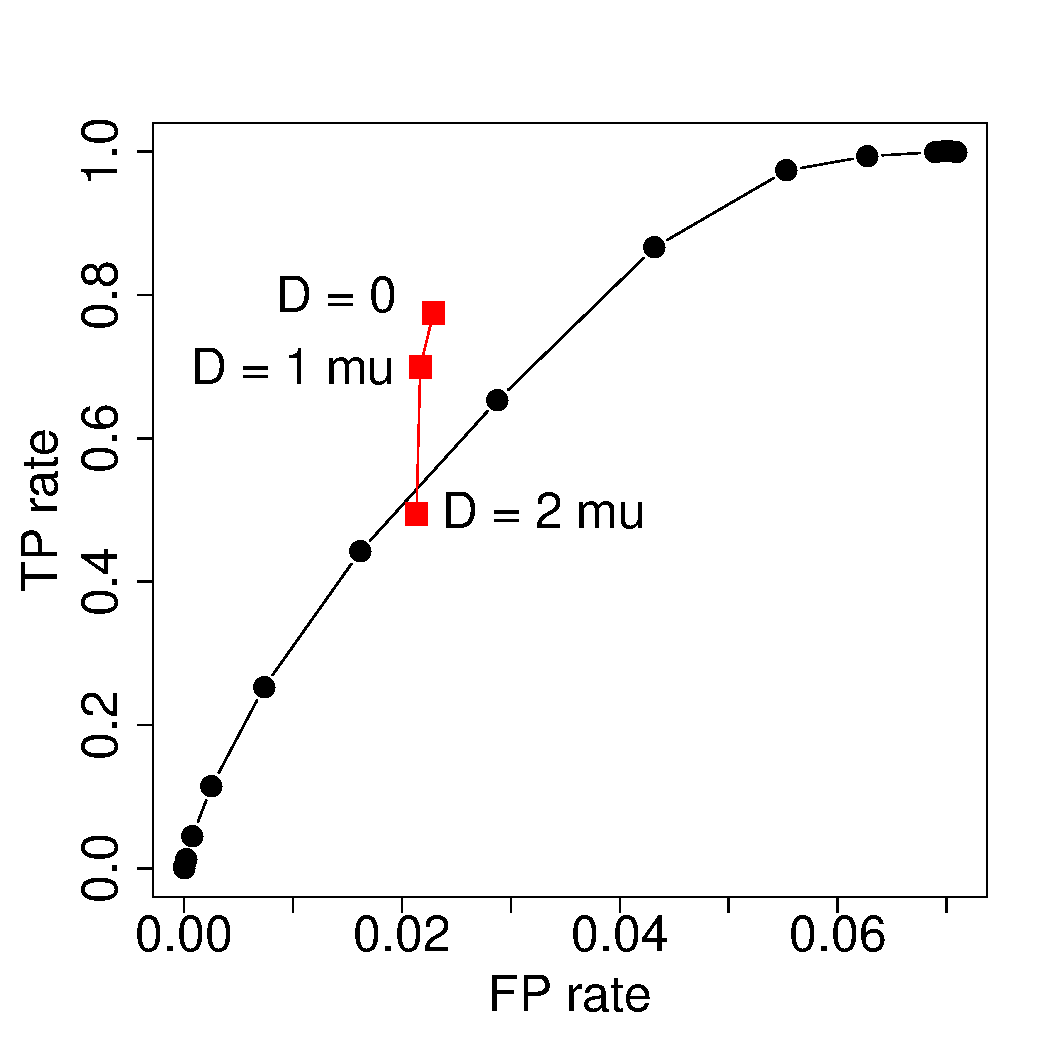
\includegraphics[width=0.30\textwidth]{articles/pics/sdm_paper/ROCImprovementAndDelay3}
\caption{
The trade-off between TPs and FPs.
Red squares show performance with the dynamic threshold with delayed feedback $(0, \mu, 2 \mu)$.}
\label{fig:rocdynamic}
\end{figure}

\subsection{Real datasets.} We experimented with two real datasets, the Boiler dataset that contains sensor readings containing recurrent refueling behavior, and the UK network traffic dataset with the typical recurrent aggregated traffic peaks.
\paragraph{Boiler dataset.}
%In this experiment we reduce FP rate of the detector used to detect changes in the real signal using PCCF in post-processing settings.
% by filtering output of the change detector.
Data comes from sensors installed on the scales measuring fuel mass in the container of Circulating Fluidized Bed boiler (CFB)~\cite{PechenizkiySIGKDDExpl09}.
%Indre: {\color{red} Data source and time of measurements, same format as in the next dataset}
The signal is shown in the top part of Figure~\ref{fig:cfbsig}, where the true changes are highlighted by vertical lines.
The mass of fuel decreases continuously as it is being consumed.
Abrupt changes in the signal happen at the start of the refueling process.
%, i.e.\ moments when new fuel is added to the container.
The signal is fluctuating due to rotating parts of the system making it difficult to distinguish the true changes from noise.

We calculated a series of PCCF,  updated after each provided confirmation with the delay $~ 2 \mu$ where $\mu$ is estimated from training data average distance between changes.
The results are shown in Figure~\ref{fig:cfbsig}.
PCCF functions are computed with confirmation delay $2\mu$ (bottom plot). Initial and updated PCCFs are marked by numbers.
Two outliers are correctly identified by PCCF and do not cause FPs.
%height = 0.35\textheight, width = 0.8\textwidth
\begin{figure}[htb!]
\centering
%\includegraphics[width = 0.8\textwidth ]{./images/new2/cfbproof2.pdf}
\includegraphics[width = 0.45\textwidth, height = 0.35\textheight, ]{articles/pics/sdm_paper/cfbproof2.pdf}
\caption{
%Outliers caused by noisy changes at the moments $t = (308, 458)$ are omitted
%The mass flow signal with abrupt changes (top) and cascades of PCCFs (bottom).
The mass flow signal with abrupt changes (top) and updated PCCFs (bottom).
Outliers due to jammed particles (vertical dashed lines) in the mass flow do not result in FPs.
}
\label{fig:cfbsig}
\end{figure}

\paragraph{The Internet traffic dataset.}
Next, we test our approach on publicly available dataset\footnote{\url{https://datamarket.com/data/list/?q=internet+traffic+data+price\%3Afree}} containing aggregated internet traffic data from Internet Service Provider in the UK academic network backbone. The data series is illustrate in Figure~\ref{fig:trafficdata}.
%\href{https://datamarket.com/data/list/?q=internet+traffic+data+price\%3Afree}{https://datamarket.com/data/list/?q=internet+traffic+data+price\%3Afree}
%Data was collected between 19 November 2004
%, at 09:30 hours
%and 27 January 2005.
%, at 11:11 hours.
Measurements were taken between 19 Nov 2004 and 27 Jan 2005  at five minute intervals.
%Signal is visualized in Figure~\ref{fig:trafficdata}.
The task is to detect on-line maximum daily traffic by detecting changes in the trend of the signal.
These changes are periodic;  we do not use information of the daytime in order to consider them as recurrent.

Figure~\ref{fig:fractraffic} shows TP and FP rates of the PCCF-based detector for post-processing settings. The results are analogues for the results obtained in the experiment on the artificial data illustrated in Figure~\ref{fig:combined}. From the left plot we can see that max delay of confirmation is $D=6\mu$.

Figure~\ref{fig:rocdynamictraffic} illustrates improvement in the performance of the detector when using PCCF.
The ROC curve (solid line) shows the trade-off between TPs and FPs of the detector. %with fixed sensitivity threshold parameter.
Each point on this curve indicates the performance of the detector with a fixed sensitivity threshold.
The red triangles depict the performance of the PCCF-based detector with post-processing corresponding to the baseline `Static' detector (denoted with a blue diamond) we chose to improve as one already having a high TP rate but poor performance wrt FPs.
The red circles depict the performance of the PCCF-based detector with post-processing settings.
Different triangles and circles correspond to different values of $D$.
The triangles and circles concentrated in the top left corner with TP rate close to $1.0$ and FP rate close to $0$ correspond to setting when $D\leq6\mu$.
When $D>6\mu$ the triangles are drifting down showing the deterioration in the TP rate.
FP rate is not increasing because in both pre- and post-processing settings of PCCF-based detector we do not generate additions CDEs as we only reduced the sensitivity of a TP-optimal static detector we chose on the ROC.
% {\color{red} What does it indicate?}
\begin{figure}[htb!]
\centering
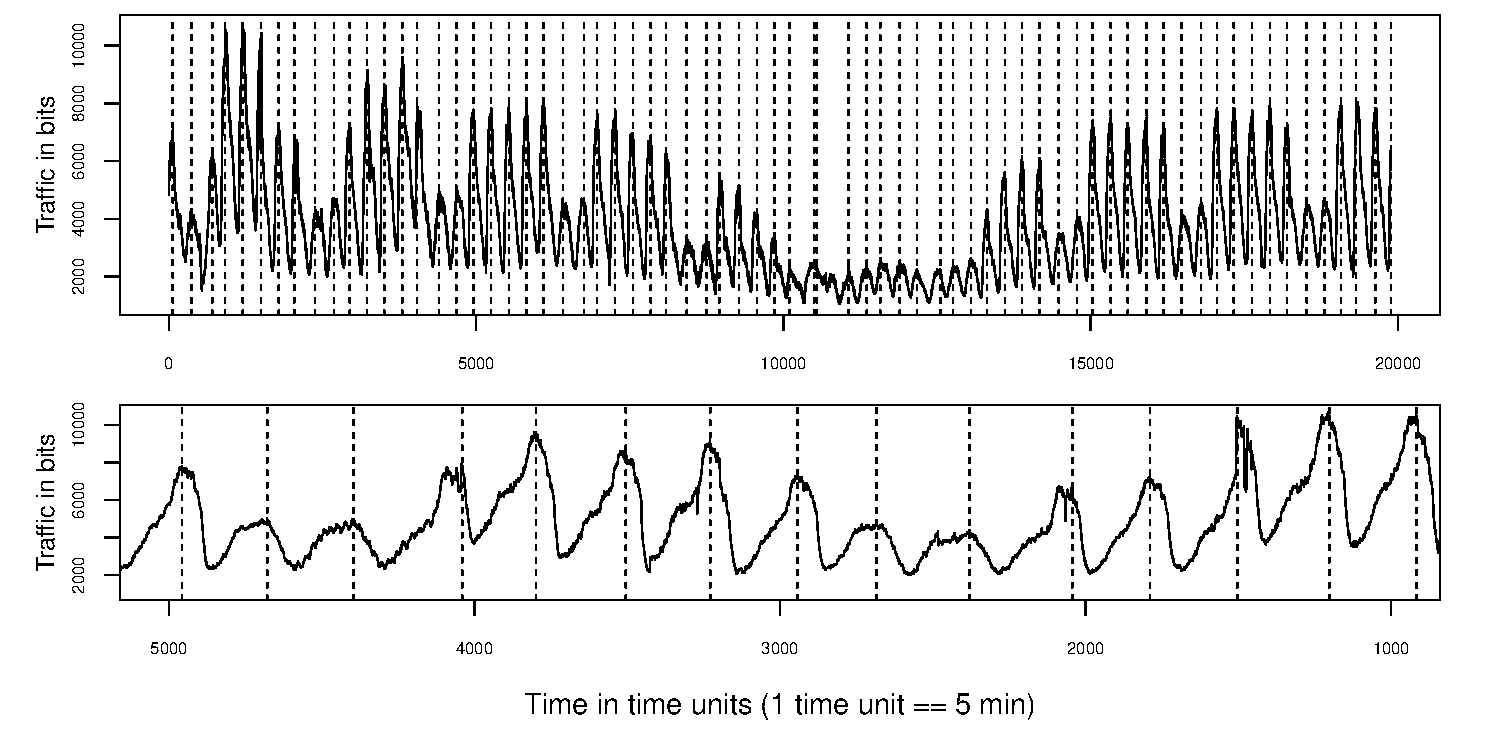
\includegraphics[width=0.48\textwidth]{articles/pics/sdm_paper/TrafficData.pdf}
\caption{
Aggregated traffic in the UK academic network.
The bottom figure in a zoomed region.
%At the bottom is enlarged part of the data.
Dashed lines depict the true change points. % to be detected are depicted by vertical dashed lines.
}
\label{fig:trafficdata}
\end{figure}
%
\begin{figure}[htb!]
\centering
%\begin{minipage}{0.35\textwidth}
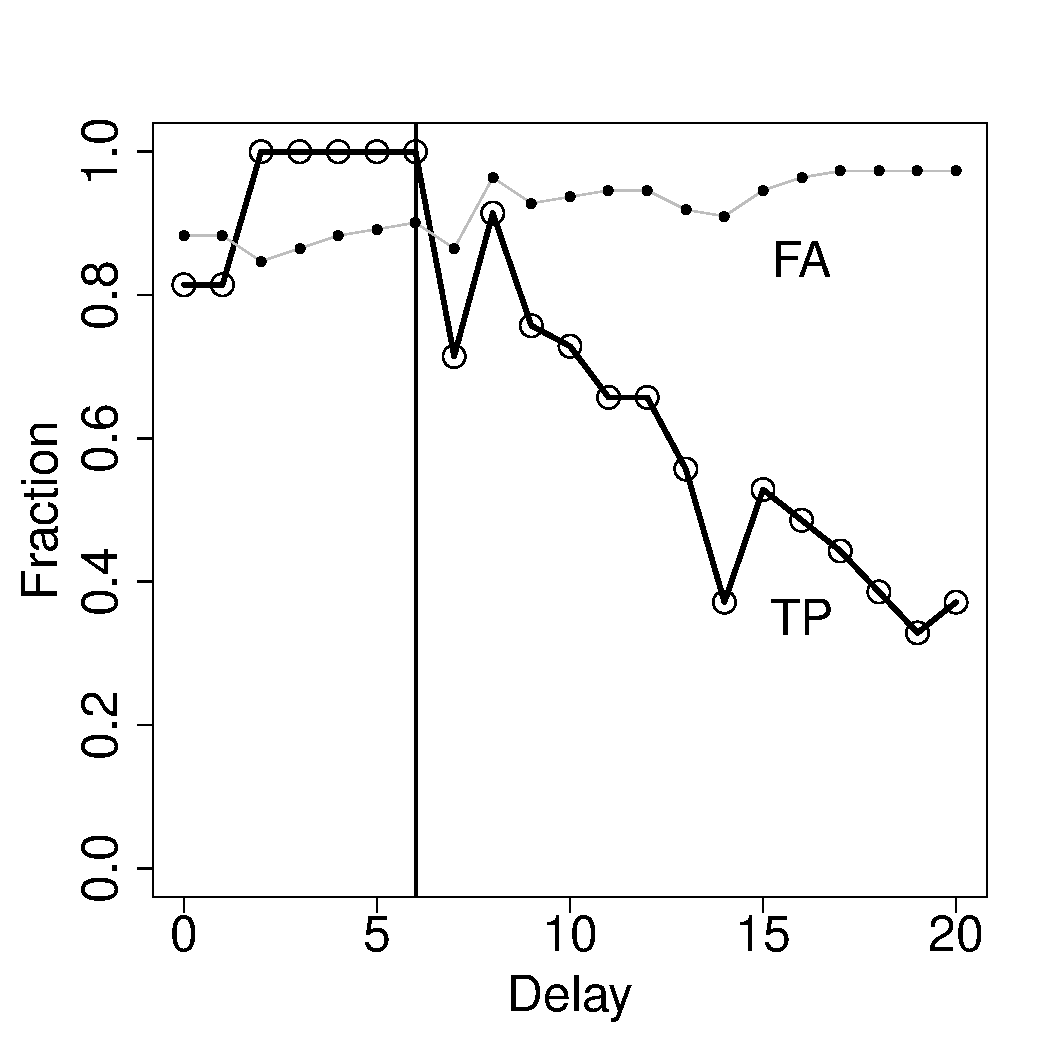
\includegraphics[width=0.24\textwidth]{articles/pics/sdm_paper/performance1sdm.pdf}
%\end{minipage}
%\begin{minipage}{0.35\textwidth}
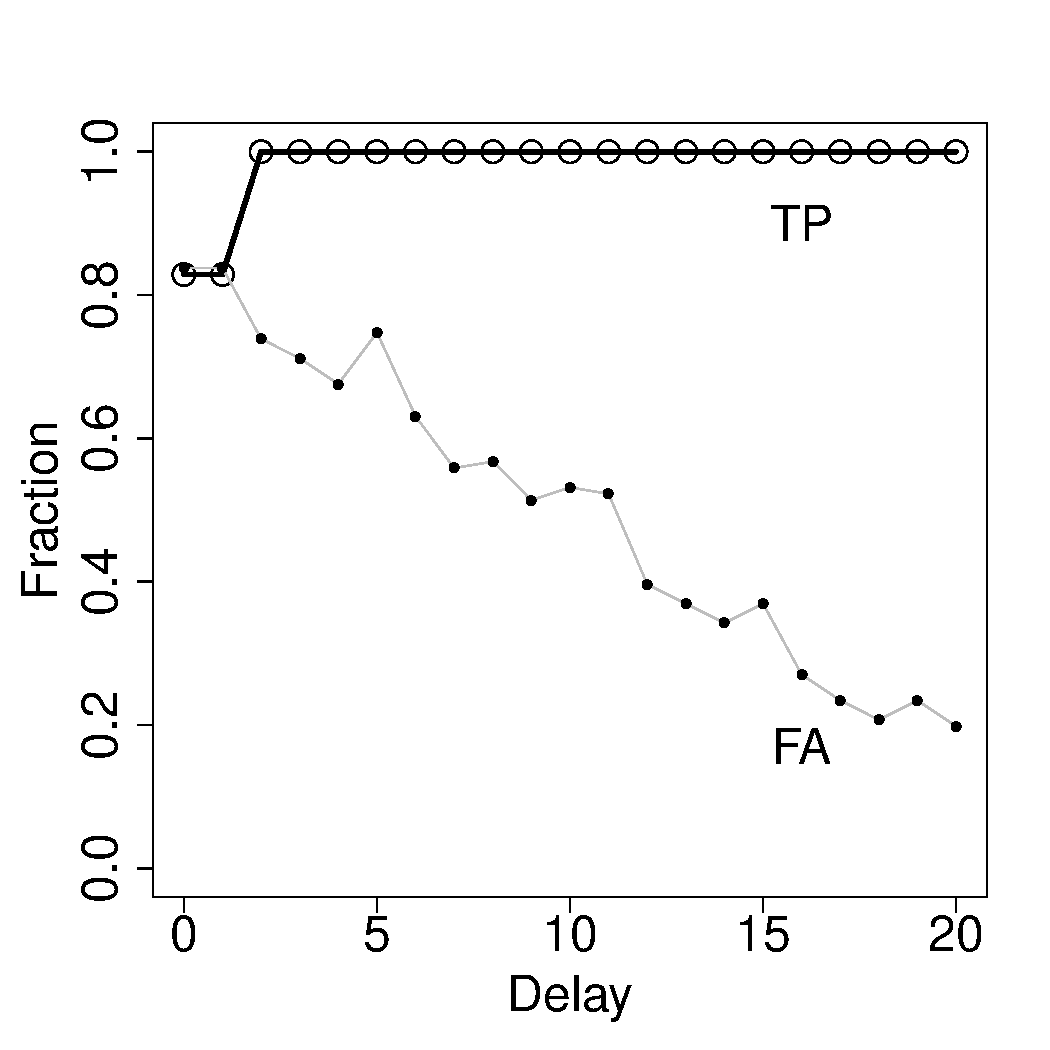
\includegraphics[width=0.24\textwidth]{articles/pics/sdm_paper/performance2sdm.pdf}
%\end{minipage}
\caption{
PCCF sensitivity and specificity for the internet traffic dataset.
Threshold is higher (left) and lower (right) than PCCF limit.
The maximum delay of confirmation is $6 \mu $ (vertical line on the left plot).
}
\label{fig:fractraffic}
\end{figure}
%
\begin{figure}[htb!]
\centering
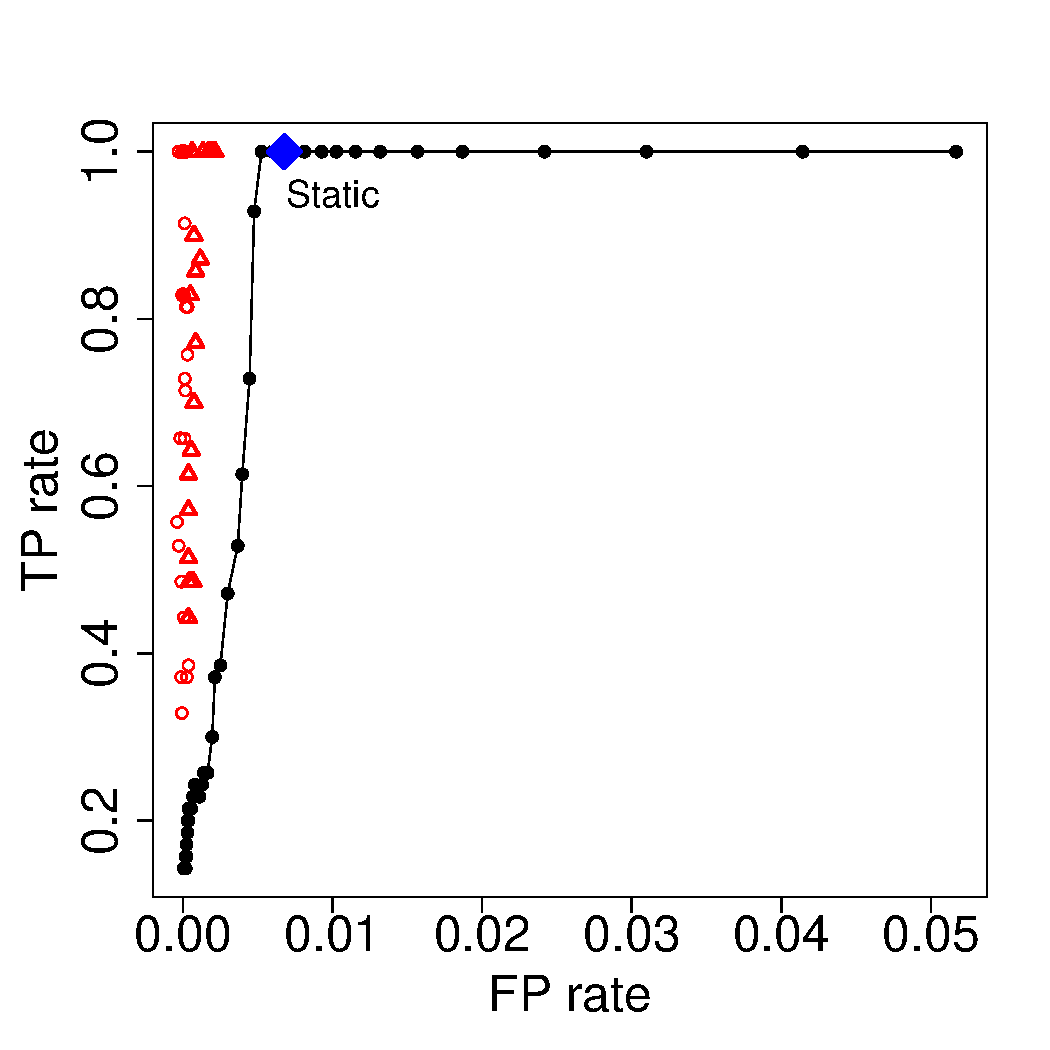
\includegraphics[width=0.3\textwidth]{articles/pics/sdm_paper/ROCimprtraff.pdf}
\caption{
	Black line - performance of the detector with static parameters.
	Red triangles - performance of PCCF based detector when applied to the  static detector with settings corresponding to the point marked as `Static'.
}
\label{fig:rocdynamictraffic}
\end{figure}

\section{Conclusions}
\label{sec:conclusions}
For handling recurrent changes we introduced the predictive change confidence function (PCCF), which is a probability mass function, conditioned on the time of the last confirmed change.
We derived the performance guarantees analytically, assuming Gaussian distribution of the time intervals between changes, and verified the analytical expression for PCCF experimentally on synthetic data.
We proved that over time values of Gaussian PCCF converge to a limit value $L = \frac{1}{\mu}$ (Eq.~\ref{eq:pccf_limit_proof}).
%We presented two simple procedures for integrating PCCF with existing change detectors, and experimentally analyzed their performance.
We demonstrated on both synthetic and real datasets the feasibility of utilizing PCCF for recurrent change detection with two simple approaches: post-processing of manifested changes and dynamic adjustment of the sensitivity of the base-level detector.

The following conclusions can be made regarding the benefits of using recurrence information for improving detections' performance:
\begin{itemize}
  \item Recurrence information $\theta=(\mu, \sigma)$ is long-term useful if limit of the PCCF $L = \frac{1}{\mu}$ when $t \to \infty$ is greater than detector error rate $\frac{1}{\mu} > \lambda$ where $\mu$ is average time between recurrent changes.
  \item Recurrence information $\theta$ is short-term useful with the max confirmation delay $D$ if local maximums of the PCCF at moments $l \mu \leq D$ after confirmed change has higher values than probability of error $\lambda$,
      %$\mathcal{P}(t \leq D) > \lambda$
      but limit $L < \lambda$.
  %\item If $\sigma$ is `high' then PCCF converges very quickly to its limit $L$ and decision is made on the basis whether its value higher or lower than the error rate $\lambda$.
  %\item If $\sigma$ is `low' then PCCF oscillates during some time and usefulness is defined by whether values of the PCCF at the moments corresponding to the local maximums $k \mu$ are higher than $\lambda$ or not.
  \item The main factor defining usefulness of $\theta$ is the ratio $\frac{\mathcal{P}(t = l \mu)}{\lambda}$ within time $D$ from the most recently confirmed change and $\frac{L}{\lambda}$ in a longer term when we do not have confirmation or $D$ is high.
\end{itemize}
%Finally, we demonstrated on two real data sets that it is possible to improve change detection performance with the proposed approach.
In the performed experiments parameters $\theta$ were assumed to be known a priory or estimated from the training data.

This work provide several straightforward opportunities for future work, in particular investigating how uncertainty of $\theta$ estimates affects the performance of recurrent change detection, and studying other approaches for integrating PCCF with different existing change detection mechanisms.

\section{Acknowledgments}
This research is partly supported by STW CAPA project and COMAS funding. We would like to thank Jaakko Hollmen and Alexander Shklyaev for useful comments on this work.
Any remaining errors are our own.

%\bibliographystyle{IEEEtran}
%\appendix
\section{PCCF pseudo-code}
\label{sec:pccf_pseudo_code}
In Algorith~1, in line 11,  a zero-matrix of size $T$ is initialized with the first column filled by initial Pmf values $p(c_1)$.
In line 12 a square lower triangular matrix (Eq.~\ref{eq:second_pccf_matrix}) is generated using the function {\tt WeightsMatrix()}.
Next the probabilities for individual changes in a sequence
$\Collect{ c_i }_{i=1}^k$
are updated within the loop (line 14).
PCCF is calculated in line 15 by summing up probabilities in the columns of matrix $P$.
\begin{algorithm}
    % CODE: Commit:  5e7cc8f, file pccf.jl -> sim1.jl
    \label{alg:pccfalg}
\begin{algorithmic}[1]
\Function{WeightsMatrix}{T,$\theta$}
	%\State n = T - i;
    \State M = zeros(T, T);  M[1, :] = 1:T
	%\State M = zeros(n, n);  M[1, :] = 1:n
	%\State M[1, :] = 1:n
	\For{i = 2:T}
		\For{j = i:T}
			\State M[i,j] = M[i-1, j-1]
		\EndFor
	\EndFor
	\State \textbf{return} Pmf($M^T$ $| \theta$)
\EndFunction
\\
\Function{PCCF}{$T, \theta=(\mu,\sigma)$}
\State P = zeros(T,T)
\State P[:,1] = Pmf(1:T $| \theta$) \Comment{Pmf fo the first change}
%\State W = Pmf(WeightsMatrix(T), $\theta$)
\State W = WeightsMatrix(T,$\theta$)
\For{i = 1:T-1}
	\State P[i+1:T,i+1]=W[1:T-i,1:T-i] * P[i:end-1, i]
	%\State Weights = WeightsMatrix(i,T)
	%\State $\text{pForward}$ = sum(Weights .* P[i,:], 2)
	%\State P[i+1,:] = vcat(zeros(i), $\text{pForward}$)
\EndFor
\State \textbf{return} sum(P,2) \Comment{Sum of columns}
\EndFunction
\end{algorithmic}
\caption{PCCF function pseudo-code}
\end{algorithm}

